% ****** Start of file OUnoise.tex ******
%%
\documentclass[%
 reprint,
%superscriptaddress,
%groupedaddress,
%unsortedaddress,
%runinaddress,
%frontmatterverbose, 
%preprint,
%showpacs,preprintnumbers,
%nofootinbib,
%nobibnotes,
%bibnotes,
 amsmath,amssymb,
 aps,
%pra,
%prb,
%rmp,
%prstab,
%prstper,
%floatfix,
]{revtex4-1}

\usepackage{graphicx}% Include figure files
\usepackage{dcolumn}% Align table columns on decimal point
\usepackage{bm}% bold math
\usepackage{subcaption}
\usepackage{float}
\usepackage{tikz}
%\usepackage{breqn}
\usetikzlibrary{calc,arrows.meta,positioning}
%\usepackage{hyperref}% add hypertext capabilities
%\usepackage[mathlines]{lineno}% Enable numbering of text and display math
%\linenumbers\relax % Commence numbering lines

%\usepackage[showframe,%Uncomment any one of the following lines to test 
%%scale=0.7, marginratio={1:1, 2:3}, ignoreall,% default settings
%%text={7in,10in},centering,
%%margin=1.5in,
%%total={6.5in,8.75in}, top=1.2in, left=0.9in, includefoot,
%%height=10in,a5paper,hmargin={3cm,0.8in},
%]{geometry}
\DeclareMathOperator\erf{erf}
\DeclareMathOperator\erfc{erfc}
\begin{document}

\preprint{APS/123-QED}

\title{Parameter estimation from an Ornstein-Uhlenbeck process with measurement noise}

\author{Helmut H. Strey}
 \affiliation{Biomedical Engineering Department and Laufer Center for Physical and Quantitative Biology, Stony Brook University, Stony Brook NY 11794-5281.}%Lines break automatically or can be forced with \\

\date{\today}% It is always \today, today,
             %  but any date may be explicitly specified

\begin{abstract}
\begin{description}
\item[PACS numbers]
May be entered using the \verb+\pacs{#1}+ command.
\end{description}
\end{abstract}

\pacs{Valid PACS appear here}% PACS, the Physics and Astronomy
                             % Classification Scheme.
%\keywords{Suggested keywords}%Use showkeys class option if keyword
                              %display desired
\maketitle

%\tableofcontents
\onecolumngrid
\subsection{Introduction}
\subsection{Probabilistic Description of Processes}
A probabilistic description of an overdamped Brownian particle in a harmonic potential (also called Ornstein-Uhlenbeck process) was first reported by Ornstein and Uhlenbeck in 1930 \cite{RN28}
\begin{equation}\label{OUp}
	x_{t+\Delta t} \sim \mathcal{N}(\mu=Bx_{t},\sigma^{2}=A(1-B^{2}))
\end{equation}
where $B(\Delta t) = \exp \left( { - \frac{\Delta t}{\tau}} \right)$ with $\tau$ as the relaxation time, and $\mathcal{N}$ representing a normal distribution.
This equation describes the conditional probability of finding a particle at time $t+\Delta t$ at $x_{t+\Delta t}$ given that it was at $x_{t}$ at time $t$.  The likelihood function for a specific time trace, that is taken at intervals $\Delta t$, $\left\{x_i(i\Delta t)\right\}$ is:
\begin{equation}
	p\left( \left\{x_i(t_i)\right\} \left| B, A \right.\right) =
	\frac{1}{\sqrt {2 \pi A} }
	\exp \left( { - \frac{{x_1}^2}{2A}}\right)
	\frac{1}{{\sqrt {2\pi A(1-B^{2}(\Delta t))}^{(N-1)} }}
	\exp \left( { - \sum\limits_{i=1}^{N-1}\frac{{{{\left( {x_{i+1} - {x_i}B(\Delta t)} \right)}^2}}}{{2A(1-B^{2}(\Delta t))}}} \right)
\end{equation}
We recently published an anlystical solution to the Ornstein-Uhlenbeck maximum likelihood problem \cite{RN91} and here we want to consider the same problem but with added noise.  For the moment, we will assume Gaussian noise that is added to each data point.  Such noise can be described as follows:
\begin{equation}
	y_{i} \sim \mathcal{N}(\mu=x_{i},\sigma=\sigma_{N})
\end{equation}
with likelihood function for the measured data $\{y_{i}\}$ given $\{x_{i}\}$ and $\sigma_{N}$:
\begin{equation}
	p\left( \left\{y_i(t_i)\right\} \left| \left\{x_i(t_i)\right\},\sigma_{N} \right.\right) =
	\frac{1}{{\sqrt {2\pi \sigma_{N}^{2}}^{N} }}
	\exp \left( { - \sum\limits_{i=1}^{N}\frac{{{{\left( {y_{i} - x_{i}B(\Delta t)} \right)}^2}}}{{2\sigma_{N}^{2}}}} \right)
\end{equation}

Since we are measuring $\{y_{i}\}$, $\{x_{i}\}$ are latent variables.  If we knew $\{x_{i}\}$ and $\{y_{i}\}$ the likelihood function would simply be.
\begin{equation}
	p\left( \{x_{i}\},\{y_{i}\}|A,B,\sigma_{N}\right) = 
	p\left( \left\{y_i(t_i)\right\} \left| \left\{x_i(t_i)\right\},\sigma_{N} \right.\right)
	p\left( \left\{x_i(t_i)\right\} \left| B, A \right.\right)
\end{equation}

\begin{figure}[H]
\begin{center}
\tikzset{
   every node/.style={font=\sffamily\small},
   main node/.style={thick,circle,draw,font=\sffamily\Large}
}
\begin{tikzpicture}[->,>={Stealth[round,sep]},shorten >=1pt,auto,node distance=2.5cm,minimum size=1.5cm]
\node[main node] (1) {$x_{1}$};
\node[main node] (2) [right of=1] {$x_{2}$};
\node[main node] (4) [right of=2] {$x_{n-1}$};
\node[main node] (5) [right of=4] {$x_{n}$};
\node[main node] (6) [right of=5] {$x_{n+1}$};
\node[main node] (8) [right of=6] {$x_{N-1}$};
\node[main node] (9) [right of=8] {$x_{N}$};
\node at ($(2)!.5!(4)$) {\ldots};
\node at ($(6)!.5!(8)$) {\ldots};

\node[main node] (10) [below of=1] {$y_{1}$};
\node[main node] (11) [below of=2] {$y_{2}$};
\node[main node] (12) [below of=4] {$y_{n-1}$};
\node[main node] (13) [below of=5] {$y_{n}$};
\node[main node] (14) [below of=6] {$y_{n-1}$};
\node[main node] (15) [below of=8] {$y_{N-1}$};
\node[main node] (16) [below of=9] {$y_{N}$};

\draw [->] (1) -- (2);
%\draw (2) -- (4);
\draw [->] (4) -- (5);
\draw [->] (5) -- (6);
\draw [->] (8) -- (9);

\draw [->] (1) -- (10);
\draw [->] (2) -- (11);
\draw [->] (4) -- (12);
\draw [->] (5) -- (13);
\draw [->] (6) -- (14);
\draw [->] (8) -- (15);
\draw [->] (9) -- (16);
\end{tikzpicture}
\caption{Graph representation of a chain of N values $\{x_{i}\}$ that originate from an OU process with corresponding $\{y_{i}\}$ that represent the measured values containing noise}\label{fig:HMCnodesfig}
\end{center}
\end{figure}

But since we don't observe $\{x_{i}\}$, we need to marginalize over $\{x_{i}\}$:
\begin{equation}
p\left( \{y_{i}\}|A,B,\sigma_{N}\right) = \idotsint p\left( \{x_{i}\},\{y_{i}\}|A,B,\sigma_{N}\right) \,dx_1 \dots dx_N
\end{equation}
Using Bayes Theorem, we can express the conditional probability of the parameters $\{A,B,\sigma_{N}\}$ given the measured data $\{y_{i}\}$.
\begin{equation}
	p\left( \{A,B,\sigma_{N}\}|\{y_{i}\},\right) =
	p\left( \{y_{i}\}|A,B,\sigma_{N}\right)p\left(A,B,\sigma_{N}\right)
\end{equation}
In principle, from this equation, we could estimate the parameters from a measurement of $\{y_{i}\}$ using a maximum likelihood approach.
\subsection{Implementation of the Expectation Maximization algorithm}
As we can see from the previous equation, a simple maximum likelihood approach is computationally challenging.  Because we are dealing with Gaussian distributions, a typical approach is to take the logarithm of the likelihood and hope that the likelihood factors nicely.  But in our case, because of the marginalization of the hidden variables $\{x_{i}\}$, we are taking the logarithm of integrals over $\{x_{i}\}$ which does not simplify the equation.  On the other hand, we recognize that $p\left( \{x_{i}\},\{y_{i}\}|A,B,\sigma_{N}\right)$ factors nicely.  The Expectation Maximization (EM) algorithm takes advantage of this fact (see \cite{RN90} chapter 9).  The EM algorithm works as follows: (1) pick a starting point for the parameters $\Theta^{old} = \{A^{old},B^{old},\sigma_{N}^{old}\}$; (2) calculate the probability distribution for each hidden variable $\{x_{i}\}$ given these parameters; (3) maximize the following function with respect to $\Theta$ to find the new parameters.
\begin{equation}
	\mathcal{Q}(\Theta,\Theta^{old}) = \idotsint p\left( \{x_{i}\}|\{y_{i}\},\Theta^{old}\right)\ln p\left( \{x_{i}\},\{y_{i}\}|\Theta\right)\,dx_1 \dots dx_N
\end{equation}
(4) repeat by using $\Theta$ as $\Theta_{old}$ until convergence.  The EM alorithm converges, but it may find local maxima in the posterior distribution.  Therefore it is important to vary the starting point for $\Theta$.  To evaluate the integral in eq., we need to calculate $p\left( x_{n}|\{y_{i}\},\Theta^{old}\right)$.  We can again use Bayes rule and the conditional indpendence rules of a linear hidden Markov chain:
\begin{equation}\label{margxn}
	\begin{aligned}
	p\left( x_{n}|\{y_{i}\},\Theta^{old}\right)&=\frac{p\left( \{y_{i}\}|x_{n},\Theta^{old}\right)p(x_{n})}{p(\{y_{i}\}|\Theta^{old})}\\
	&=\frac{p(y_{1},\dots,y_{n}|x_{n},\Theta^{old})p(y_{n+1},\dots,y_{N}|x_{n},\Theta^{old})p(x_{n})}{p(\{y_{i}\}|\Theta^{old})}\\
	&=\frac{p(y_{1},\dots,y_{n},x_{n}|\Theta^{old})p(y_{n+1},\dots,y_{N}|x_{n},\Theta^{old})}{p(\{y_{i}\}|\Theta^{old})}
	&=\frac{\alpha(x_{n})\beta(x_{n})}{p(\{y_{i}\}|\Theta^{old})}
	\end{aligned}
\end{equation}
using the following definition
\begin{equation}
	\begin{aligned}
	\alpha(x_{n})&=p(y_{1},\dots,y_{n},x_{n}|\Theta^{old})\\
	\beta(x_{n})&=p(y_{n+1},\dots,y_{N}|x_{n},\Theta^{old})
	\end{aligned}
\end{equation}
here we took advantage of the properties of the Markov chain $\{x_{i}\}$.  If we know a specific $x_{n}$ then $x_{n-1}$ and $x_{n+1}$ are independent because the path between the two is blocked (See for example \cite{RN90}).  As a consequence of that, the $y_{i}$ with $i\leq n$ are independent of $y_{i}$ with $i>n$ conditioned on $x_{n}$.  Both $\alpha(x_{n})$ and $\beta(x_{n})$ can be defined and calculated recursively:
\begin{equation}
	\begin{aligned}
	\alpha(x_{n})&=p(y_{n}|x_{n},\Theta^{old})\int \alpha(x_{n-1})p(x_{n}|x_{n-1},\Theta^{old})dx_{n-1}\\
	\beta(x_{n})&=\int \beta(x_{n+1})p(y_{n+1}|x_{n+1},\Theta^{old})p(x_{n+1}|x_{n},\Theta^{old})dx_{n+1}
	\end{aligned}
\end{equation}
with the starting value of
\begin{equation}
	\begin{aligned}
\alpha(x_{1})&\propto \exp \left( { - \frac{{x_1}^2}{2A}}\right)\exp \left( -\frac{{{{\left( {y_{1} - x_{1}} \right)}^2}}}{{2\sigma_{N}^{2}}} \right)\\
\beta(x_{N})&=1
	\end{aligned}
\end{equation}
Here we have to notice that all probabiltiy distributions are Gaussian, which means that the product of two Gaussians as well as the convolution of two Gaussians is also a Gaussian.  As a consequence, all $\alpha(x_{n})$ and $\beta(x_{n})$ are Gaussian (except for $\beta(x_{N})$).  For a computation, all we need to calculate is the mean and standard deviation of each $\alpha(x_{n})$ and $\beta(x_{n})$ since the normalization of Gaussians is known.  Similarily, we can calculate the probability distributions of consecutive $x_{n-1}$ and $x_{n}$:
\begin{equation}\label{margxnxnmone}
	\begin{aligned}
	p\left( x_{n-1},x_{n}|\{y_{i}\},\Theta^{old}\right)&=\frac{p\left( \{y_{i}\}|x_{n-1},x_{n},\Theta^{old}\right)p(x_{n-1},x_{n})}{p(\{y_{i}\}|\Theta^{old})}\\
	&=\frac{p(y_{1},\dots,y_{n}|x_{n},\Theta^{old})p(y_{n+1},\dots,y_{N}|x_{n},\Theta^{old})p(x_{n})}{p(\{y_{i}\}|\Theta^{old})}\\
	&=\frac{\alpha(x_{n-1})p(y_{n}|x_{n},\Theta^{old})p(x_{n}|x_{n-1},\Theta^{old})\beta(x_{n})}{p(\{y_{i}\}|\Theta^{old})}
	\end{aligned}
\end{equation}
We can now move to the implementation of the EM algorithm for our specific case: (1) We pick starting values for the parameters ${A,B,\sigma_N}$; (2) We calculate all $p\left( x_{n}|\{y_{i}\},\Theta^{old}\right)$ and $p\left( x_{n-1},x_{n}|\{y_{i}\},\Theta^{old}\right)$ which represent the E step; (3) We calculate the improved parameters by using the procedure for estimating parameters from a OU process without noise \cite{RN91}, which yields improved parameters for $A$ and $B$.  For this analysis we only require the expectation values of $x_{1}^{2},x_{N}^2$, the sum of $x_{i}^2$, and $x_{i}x_{i+1}$ which can be calculated using eq.\ref{margxn} and eq.\ref{margxnxnmone}.  The updated value for $\sigma_{N}$ can be obtained by considering the following:
\begin{equation}
	\ln \prod_{i=1}^{N}\frac{1}{\sqrt{2\pi\sigma_{N}^{2}}}\exp\left(-\frac{(x_{i}-y_{i})^2}{2\sigma_{N}^{2}}\right)=-N\ln\sigma_{N}-\frac{1}{2\sigma_{N}^2}\sum_{i=1}^{N}(x_{i}-y_{i})^2
\end{equation}
The maximum of this expression can be found by setting its derivative with respect to $\sigma_N$ to zero, which results in:
\begin{equation}
	\sigma_{N, max}^{2} = \frac{1}{N}\sum_{i=1}^{N}\sigma_{x_{i}}^{2}+\mu_{x_{i}}^{2}+y_{i}^{2}-2\mu_{x_{i}}y_{i}
\end{equation}
where we use the $\sigma_{x_{i}}$ and $\mu_{x_{i}}$ from $p\left( x_{n}|\{y_{i}\},\Theta^{old}\right)=\mathcal{N}(x_{i},\mu=\mu_{x_{i}},\sigma=\sigma_{x_{i}})$.\\
To determine the error of the estimated parameters after convergence of the EM algorithm, we can take advantage of the fact that when the EM algorithm has converged then $\mathcal{Q}(\Theta,\Theta^{old})$ is equal to the posterior distribution \cite{RN90} and we can use the error estimates for $A$ and $B$ from \cite{RN91}. Since $\sigma_{N}$ is independent from $A$ and $B$ in $\mathcal{Q}(\Theta,\Theta^{old})$, we can write:
\begin{equation}
	d\sigma_{N,max} = \frac{\sigma_{N, max}}{\sqrt{2N}}
\end{equation}
\subsection{Validation with Simulations}
In this section we will validate our EM algorithm against Markov-Chain Monte-Carlo (MCMC) methods using simulated ground truth OU time series with known parameters. MCMC methods are drawing samples directly from the posterior distribution and therefore provide accurate estimations of the parameters and their uncertainties.  The expectation is that our EM algoritm will perform equally well as the MCMC methods while providing a significant computational speed increase.
\begin{figure}[H]
\begin{center}
\resizebox{.9\textwidth}{!}{%
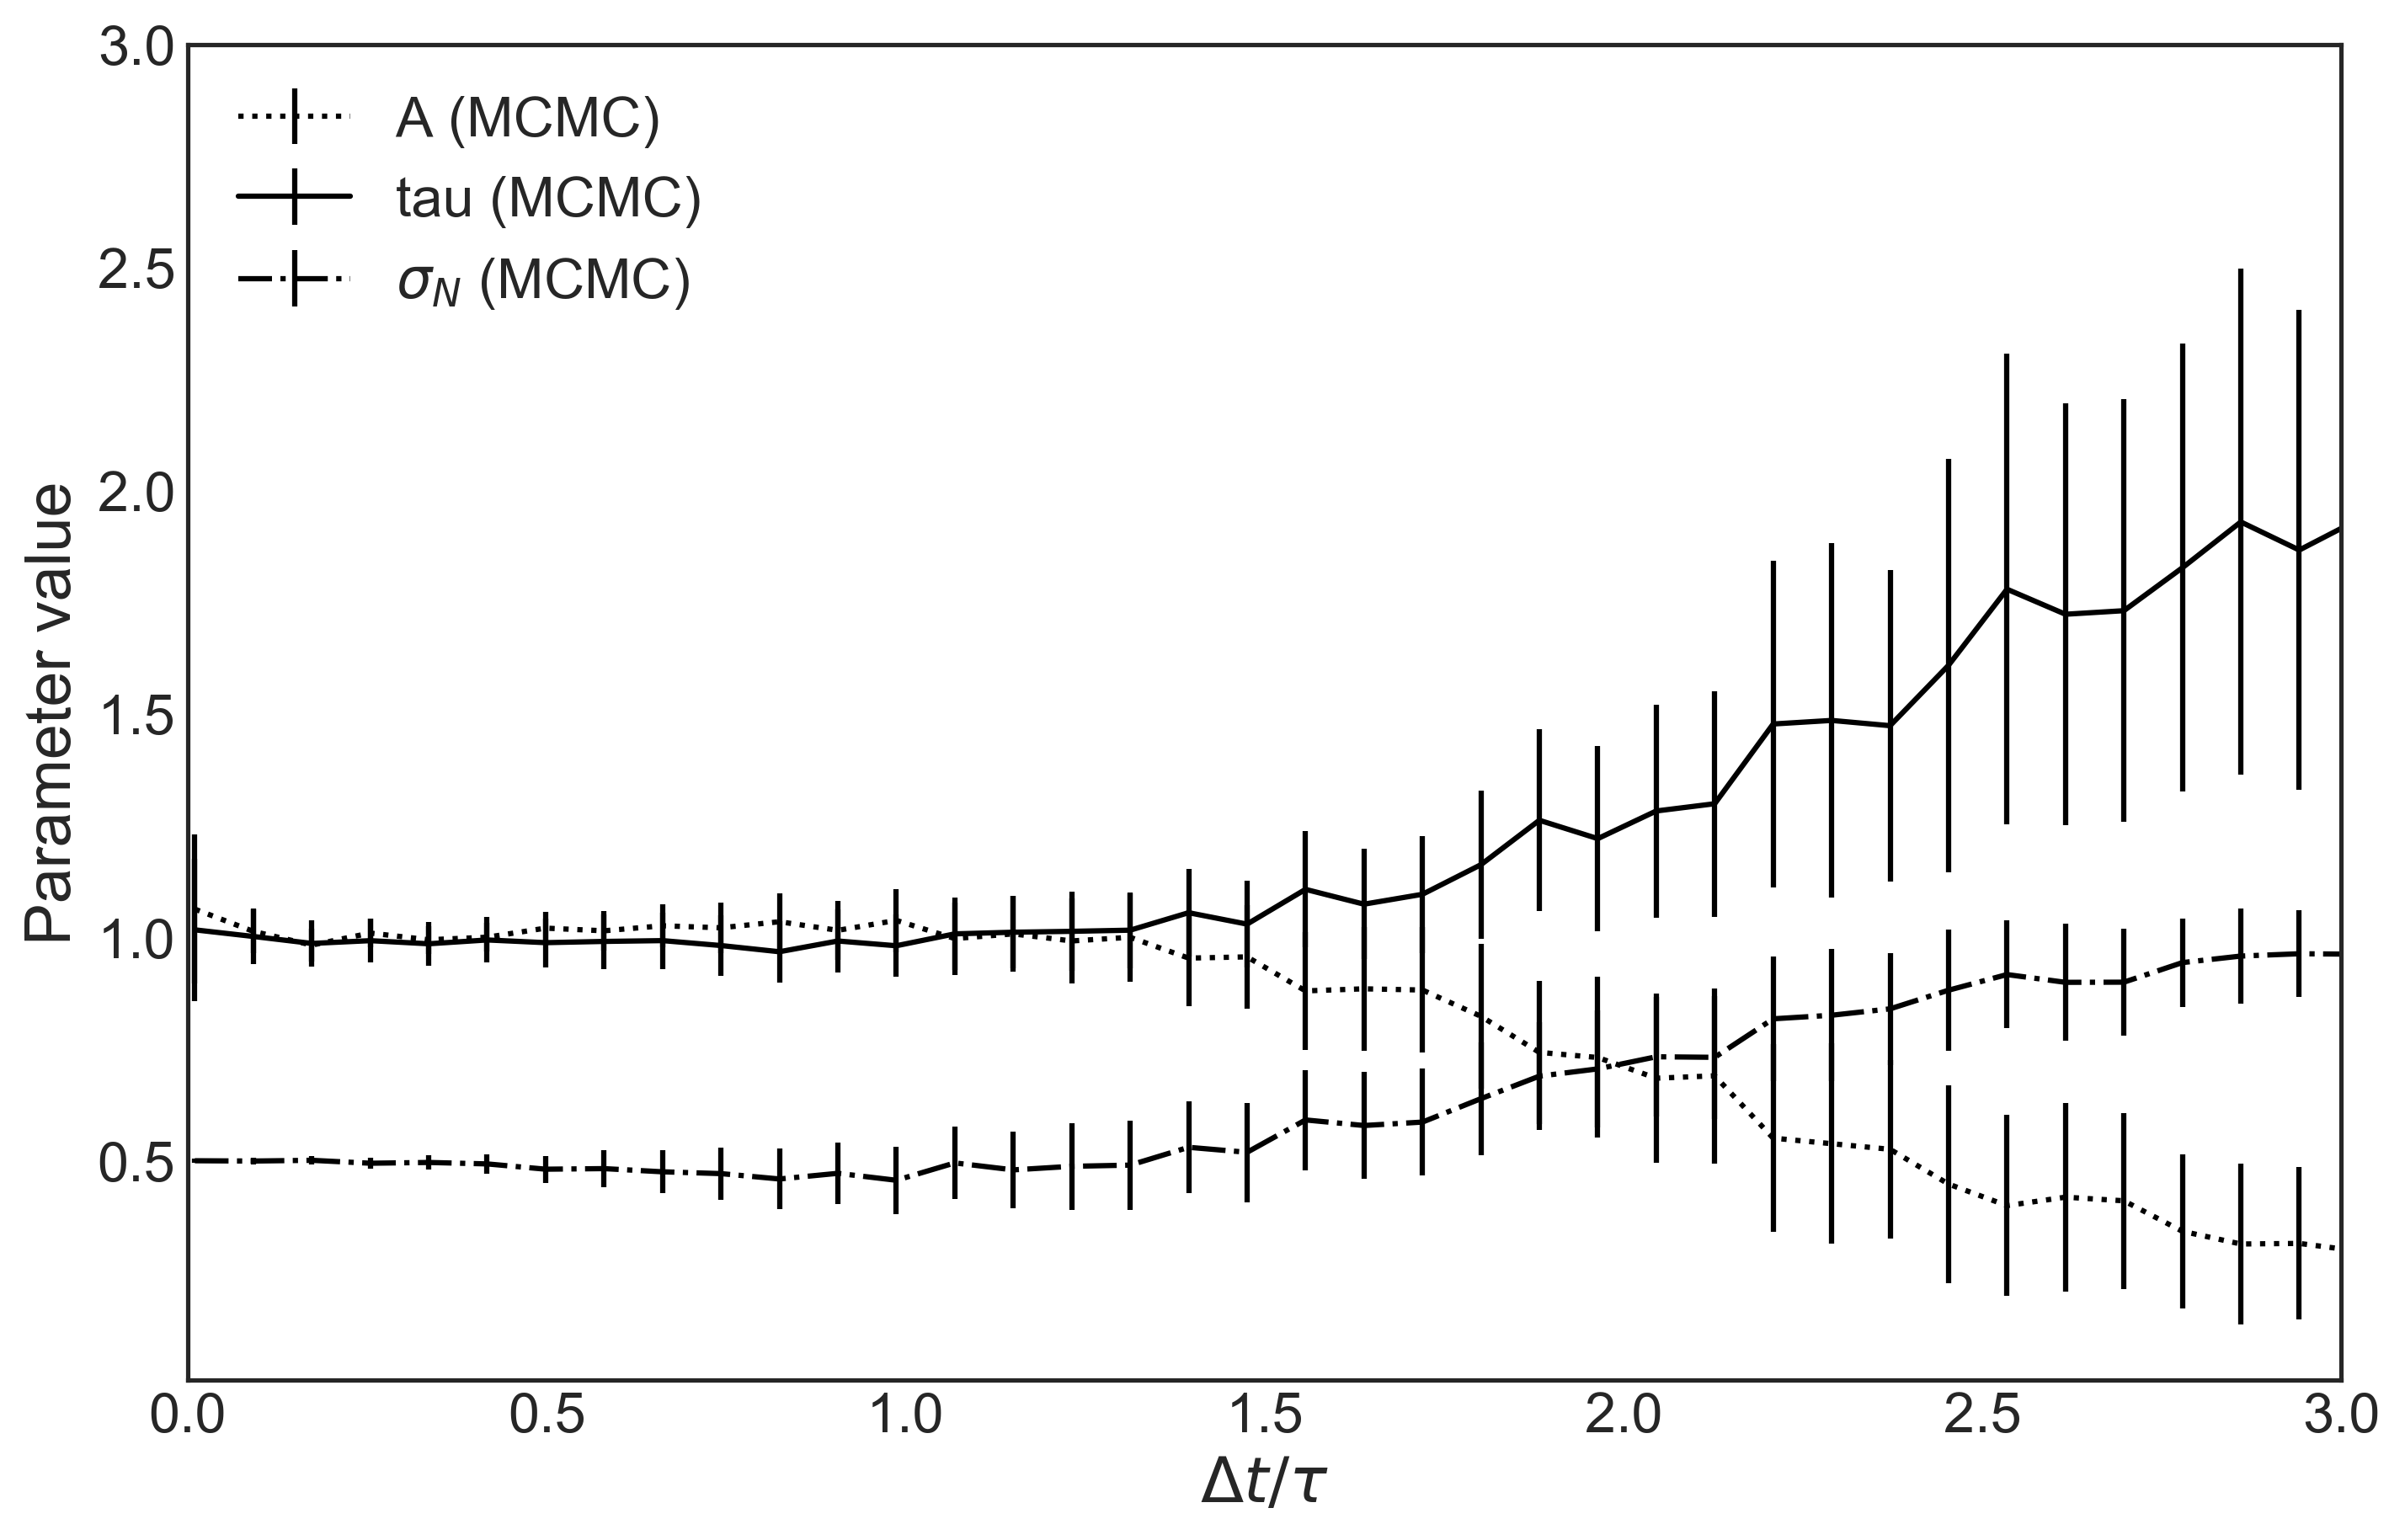
\includegraphics[height=3cm]{MCMCmultitau.png}%
\quad
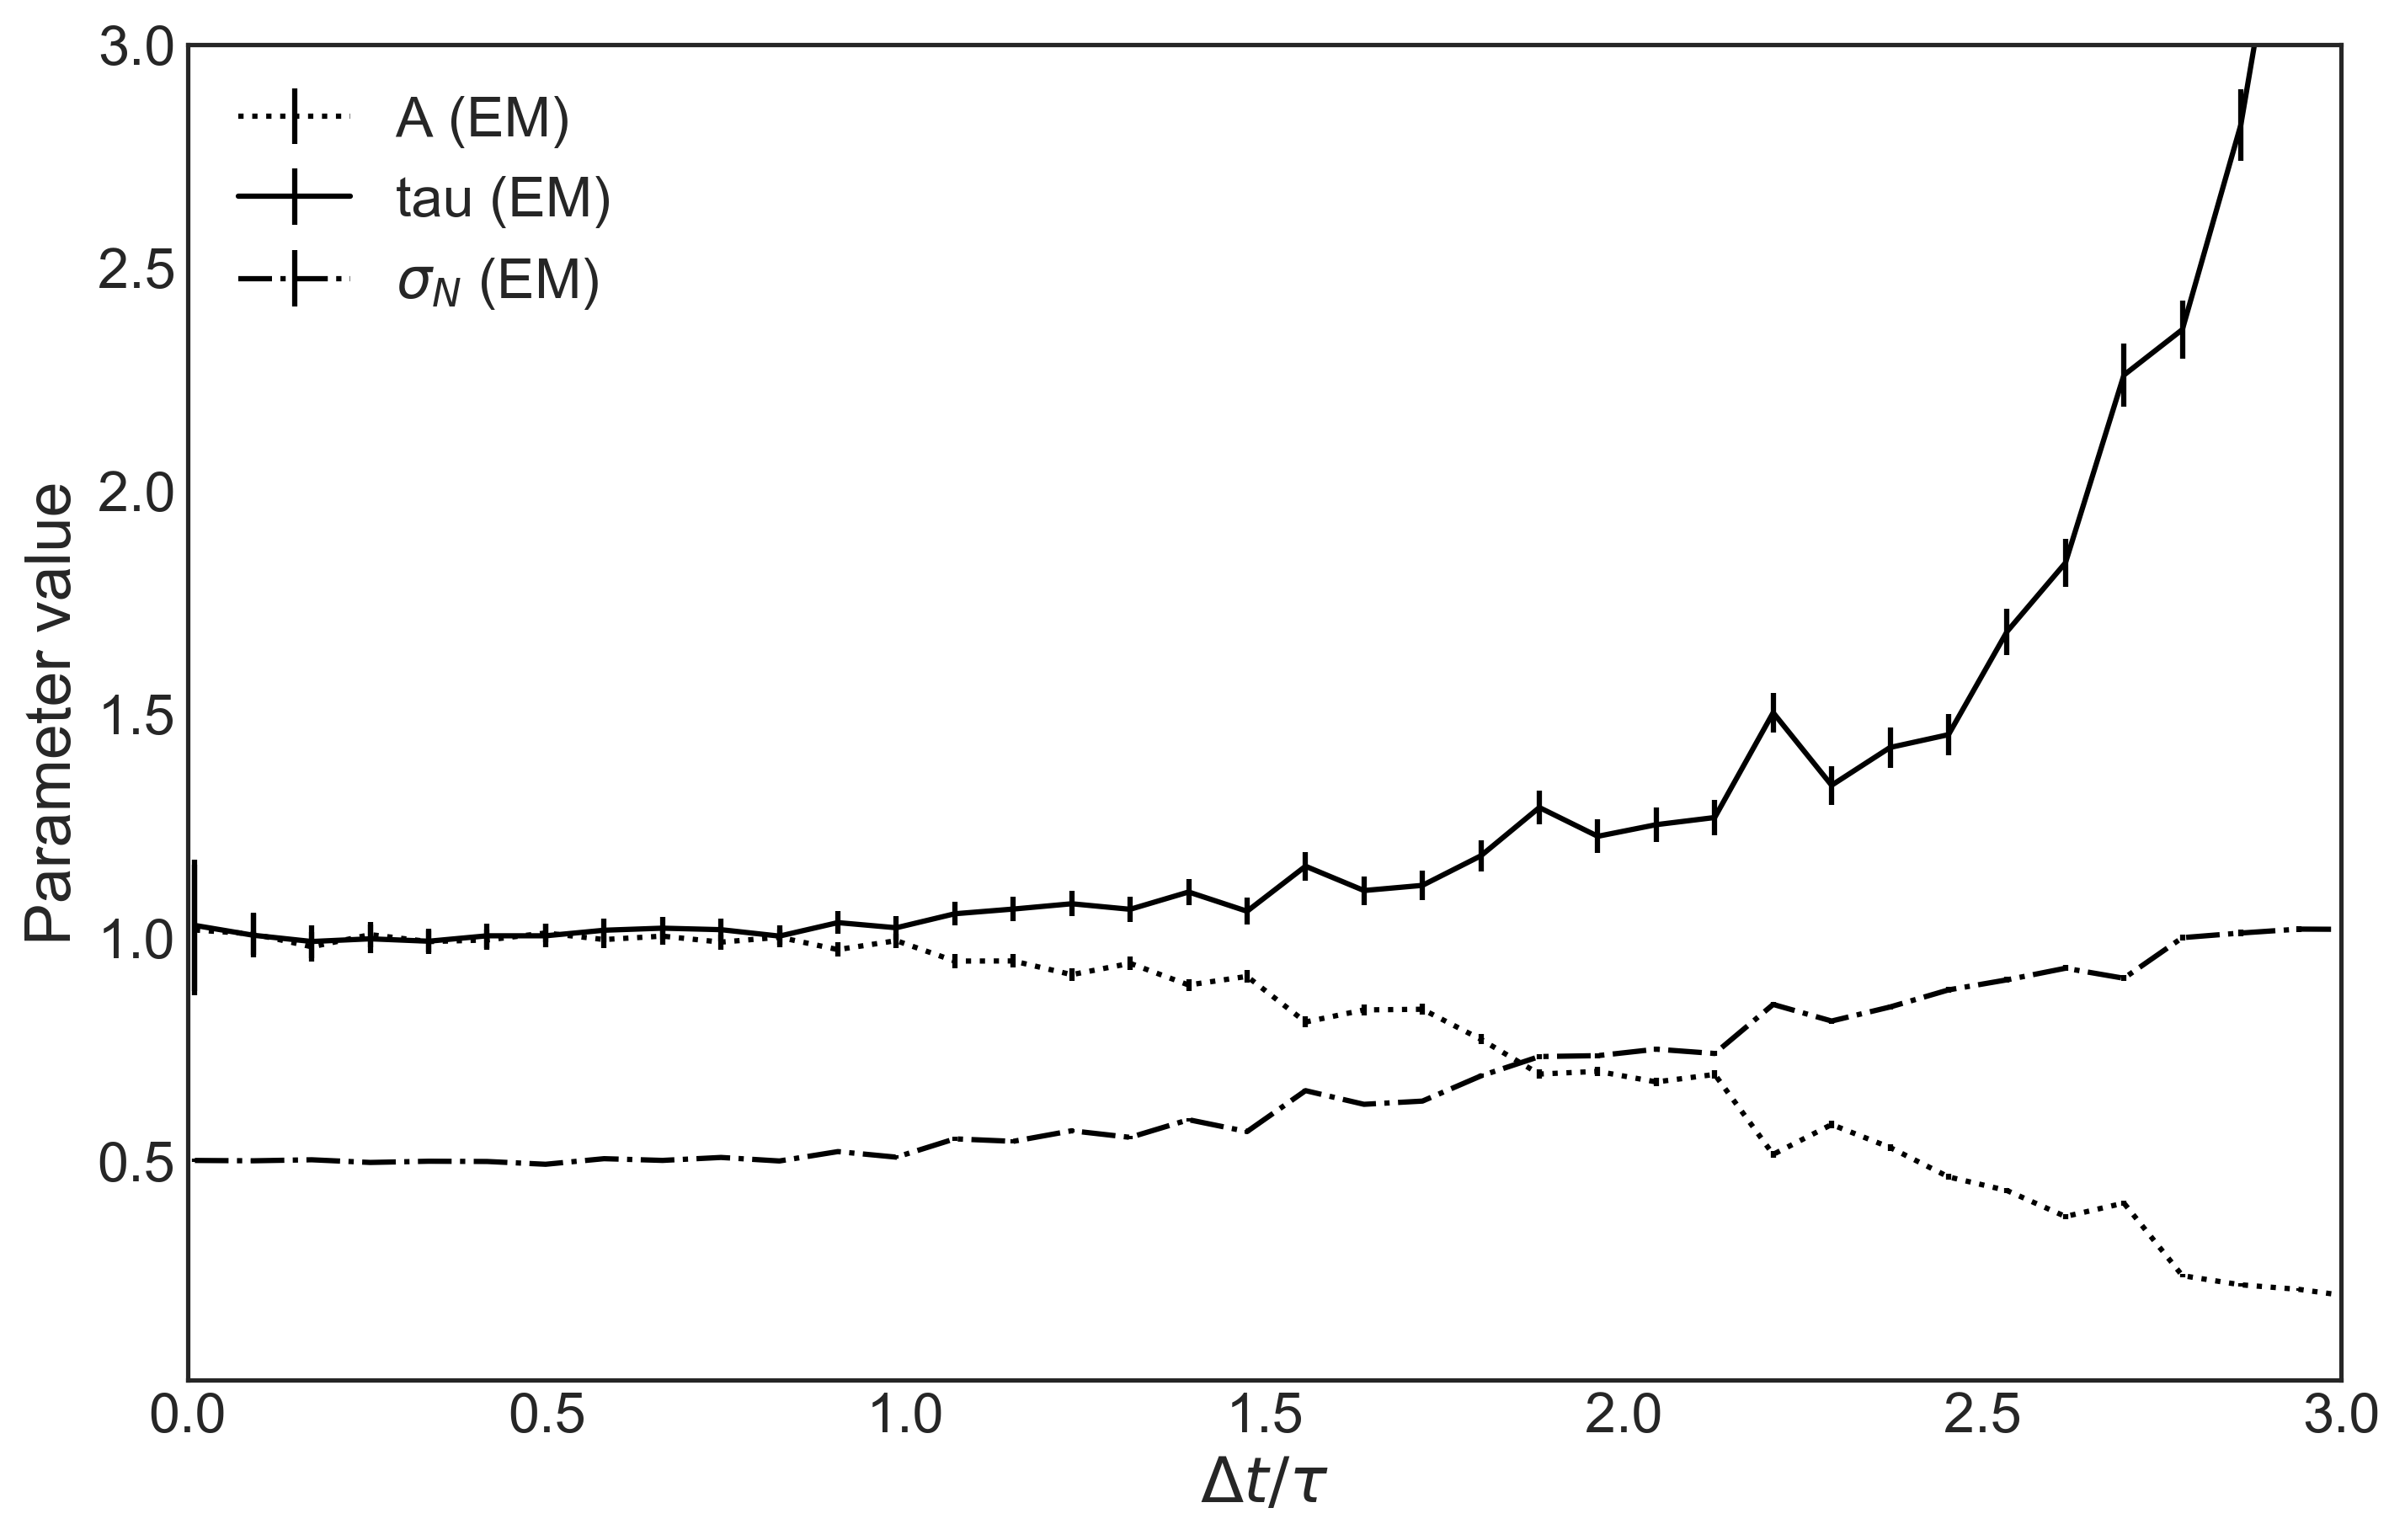
\includegraphics[height=3cm]{EMmultitau.png}%
}
\caption{}\label{fig:multitau}
\end{center}
\end{figure}

\subsection{Appendix}
In this section we collect useful procedures for calculating the different steps in the EM algorithm.
\subsubsection{Product of two Gaussians}
\begin{equation}
\mathcal{N}(x,\mu_{1},\sigma_{1})\mathcal{N}(x,\mu_{2},\sigma_{2}) 
\propto \mathcal{N}\left(x,\frac{\mu_{1}\sigma_{2}^{2}+\mu_{2}\sigma_{1}^{2}}{\sigma_{1}^2+\sigma_{2}^2},\sqrt{\frac{\sigma_{1}^2\sigma_{2}^2}{\sigma_{1}^2+\sigma_{2}^2}}\right)
\end{equation}
\subsubsection{Convolution of two Gaussians}
\begin{equation}
\int_{-\infty}^{+\infty}\mathcal{N}(x-y,\mu_{1},\sigma_{1})\mathcal{N}(y,\mu_{2},\sigma_{2})dy
	\propto\mathcal{N}\left(x,\mu_{1}+\mu_{2},\sqrt{\sigma_{1}^2+\sigma_{2}^2}\right)
\end{equation}
specifically, to calculate $\alpha(x_{n})$ and $beta(x_{n-1})$ we encounter the following convolutions
\begin{equation}
	\begin{aligned}
	\int_{-\infty}^{+\infty}dx_{n-1}
	\exp \left( -\frac{{{{\left( {x_{n-1} - \mu} \right)}^2}}}{{2\sigma^{2}}} \right)
	\exp \left( -\frac{{{{\left( {x_{n} - Bx_{n-1}} \right)}^2}}}{{2A(1-B^{2})}} \right)
	&\propto \mathcal{N}\left(x_{n},B\mu,\sqrt{B^{2}\sigma^2+A(1-B^{2})}\right)\\
	\int_{-\infty}^{+\infty}dx_{n}
	\exp \left( -\frac{{{{\left( {x_{n} - y_{n}} \right)}^2}}}{{2\sigma_{N}^{2}}} \right)
	\exp \left( -\frac{{{{\left( {x_{n} - Bx_{n-1}} \right)}^2}}}{{2A(1-B^{2})}} \right)
	&\propto \mathcal{N}\left(x_{n-1},y_{n}/B,\sqrt{\sigma^2+A(1-B^{2})}/B\right)
	\end{aligned}
\end{equation}
\subsubsection{Calculate crosscorrelation coefficients}
In Eq. \ref{margxnxnmone} we encounter bivariate distributions such as
\begin{equation}
	\begin{aligned}
	p(x,y)=\frac{1}{S}
%	\frac{1}{2\pi}\sqrt{\frac{B^{2}}{A(1-B^{2})}+\frac{1}{\sigma_{x}^{2}}}\sqrt{\frac{1}{A(1-B^{2})+B^{2}\sigma_{x}^{2}}}
%	\exp\left( \frac{(\mu_{y}-B\mu_{x})^{2}}{2(A(1-B^{2})+B^{2}\sigma^{x}_{x}+\sigma^{2}_{y})}\right)\\
	\exp \left( -\frac{{{{\left( {x - \mu_{x}} \right)}^2}}}{{2\sigma_{x}^{2}}} \right)
	\exp \left( -\frac{{{{\left( {y - Bx} \right)}^2}}}{{2A(1-B^{2})}} \right)
	\exp \left( -\frac{{{{\left( {y - \mu_{y}} \right)}^2}}}{{2\sigma_{y}^{2}}} \right)
	\end{aligned}
\end{equation}
where $S$ is the normalization constant
\begin{equation}
	S = \int_{-\infty}^{\infty}\int_{-\infty}^{\infty}p(x,y)dxdy
\end{equation}
resulting in the expectation value of $xy$
\begin{equation}
	\begin{aligned}
	\mathbb{E}(xy) &= \int_{-\infty}^{\infty}\int_{-\infty}^{\infty}p(x,y)xydxdy\\
	&=	\frac{1}{(A(1-B^{2})+B^{2}\sigma^{x}_{x}+\sigma^{2}_{y})^{2}}\\
&\left( A(1-B^{2})(B^{2}\mu_{x}\mu_{y}\sigma_{x}^{2}+B\mu_{y}^{2}\sigma_{x}^{2}+\mu_{x}\mu_{y}\sigma_{y}^{2}+B(\mu_{x}^{2}+\sigma_{x}^{2})\sigma_{y}^{2})\right.\\
	&\left.+B(2B\mu_{x}\mu_{y}\sigma_{x}^{2})\sigma_{y}^{2}+(\mu_{x}^{2}+\sigma_{x}^{2})\sigma_{y}^{2}+B^{2}\sigma_{x}^{2}(\mu_{y}^2+\sigma_{y}^{2}))
	+A^{2}(1-B^{2})^{2}\mu_{x}\mu_{y} \right)
	\end{aligned}
\end{equation}
\begin{acknowledgments}
We wish to acknowledge funding by the 
\end{acknowledgments}
\bibliography{OUnoise}
\end{document}
